% !TeX root = DistributedConsensus.tex
% !TeX spellcheck = en_GB
\chapter{Connecting Histories} 
\label{chap:connecting-histories}
	After determining how to represent histories, we want to combine actions from multiple into one history. This chapter defines the this merging of actions.
	
    \newpar
    Given a set of local histories, we want to connect the actions of the histories such that the result has the fewest possible concurrent actions. 
    
    Furthermore, given a global history $A$ and every local history $B$ used for the creation of $A$, for every path from action $x$ to another action $y$ in $B$, there must also exist a path from $x$ to $y$ in $A$.
    
    \figuretodo{Jeg ved ikke om det er for komplekst at starte med. Men man kan godt lave en figur der præsenterer det ønskede resultat.}
    
    \newpar
    The concept of happens-before relations, as described in \autoref{subsec:orderingofevents} helps determining what actions have happened before others across events.
	
    \newpar
	Actions can form pairs according to their action types. Action types 1 through 8 in \autoref{def:actiontype} represent the two sides of actions of the same message exchange.
	
	\begin{itemize}
		\item \textit{Outgoing action types} are action types \ref{actiontype:includes}, \ref{actiontype:excludes}, \ref{actiontype:setspending}, and \ref{actiontype:checkscondition}.
		\item \textit{Incoming action types} are action types \ref{actiontype:includedby}, \ref{actiontype:excludedby}, \ref{actiontype:setpendingby}, and \ref{actiontype:checkedconditionby}. 
	\end{itemize}
		
	\noindent Each outgoing action type corresponds to an incoming action type by the following definition:
	
	\begin{definition}
		\label{def:happensbeforeaction}
		The action types that \textbf{correspond} are:
			\begin{itemize}
				\item Includes $\rightarrow$ Included by
				\item Excludes $\rightarrow$ Excluded by
				\item Sets pending $\rightarrow$ Set pending by
				\item Checks condition $\rightarrow$ Checked condition by
			\end{itemize}
	\end{definition}
	
	\noindent For readability an \textit{outgoing action} is an action with an outgoing action type. In the same fashion an \textit{incoming action} is an action with an incoming action type.
	
	\newpar For any action on an event with action type 1 through 8, there might exist any number of actions with corresponding action types. However, because a pair of actions are part of the same message exchange, there is only one corresponding action.
	
	Actions should therefore be matched on more than just their corresponding action type. An action includes the ID and timestamp of both the performing and counterpart event to ensure that matches are unique.
    Pairs of actions correspond if they share a corresponding type, while the ID and timestamp of either action matches the counterpart ID and timestamp of the other.\figuretodo{Igen, måske for meget. Men man kunne godt lave en figur hvor man først matcher en action med alle andre actions der har corresponding action types, og på anden del af figuren viser at der kun er ét korrekt match.}
    
    \begin{definition}
    	\label{def:action:matching}
    	A pair of actions, $a$ and $b$, \textit{\textbf{matches}} if and only if they have corresponding action types and the ID and timestamp of $a$ is identical with the counterpart ID and counterpart timestamp of $b$. Also the ID and timestamp of $b$ must be identical with the counterpart ID and counterpart timestamp of $a$.
    \end{definition}
    
    \begin{figure}[H]
		\centering
		\begin{minipage}{0.45\textwidth}
			\centering
			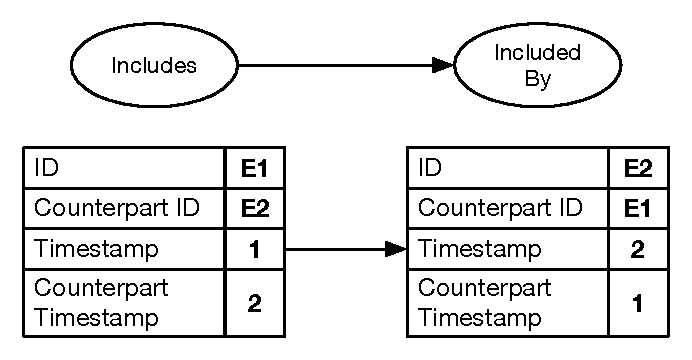
\includegraphics[width=\textwidth]{4connect/images/actions-match.pdf}
		\caption{Two actions that match.}
		\label{fig:connect:actions-match}
		\end{minipage}\hfill
		\begin{minipage}{0.45\textwidth}
			\centering
			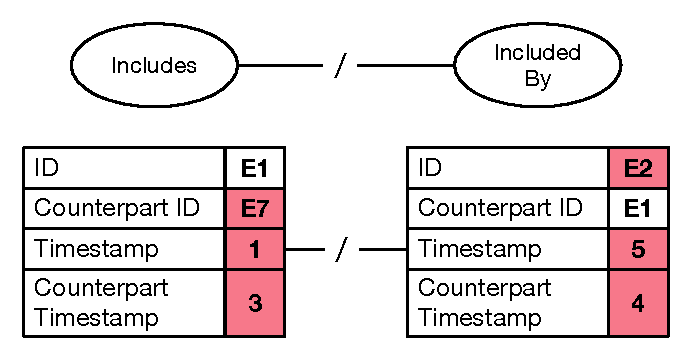
\includegraphics[width=\textwidth]{4connect/images/actions-do-not-match.pdf}
		\caption{Two actions that do not match. Fields that do not match are marked with red.}
		\label{fig:connect:actions-do-not-match}
		\end{minipage}
		\end{figure}
    
    \newpar An outgoing action must happen before its incoming counterpart, because they together represent a message exchange between to processes. A happens before relation is established between the matching actions. Therefore an edge can be added from the outgoing action to the incoming action in a history.

	\newpar To create a history of the entire set of events, every action of every local history needs to be added to a joined history. Whenever a pair of matching actions are found the edge is added from the performing action to the counterpart action. With this algorithm a set of histories can then be merged together, two at a time, until one final combined history remains. The \textit{Merge} algorithm is outlined in \autoref{alg:merge}.
	
	\begin{algorithm}
		\begin{algorithmic}
			\Function{Merge}{history1, history2}
			\State combinedHistory $\leftarrow$ \Call{UnionNodesAndEdges}{history1, history2}
			\ForAll{action \textit{in} combinedHistory}
			\If{\Call{IsOutgoing}{action}}
			\State match $\leftarrow$ \Call{FindMatchingAction}{action, combinedHistory}
			\If{\Call{IsNotNull}{match}}
			\State combinedHistory $\leftarrow$ \Call{AddEdge}{action, match, combinedHistory}
			\EndIf
			\EndIf
			\EndFor
			\State\Return combinedHistory
			\EndFunction
		\end{algorithmic}
		\caption{The \textit{\textbf{Merge}} algorithm}
		\label{alg:merge}
	\end{algorithm}
	
	\begin{figure}[H]
		\centering
		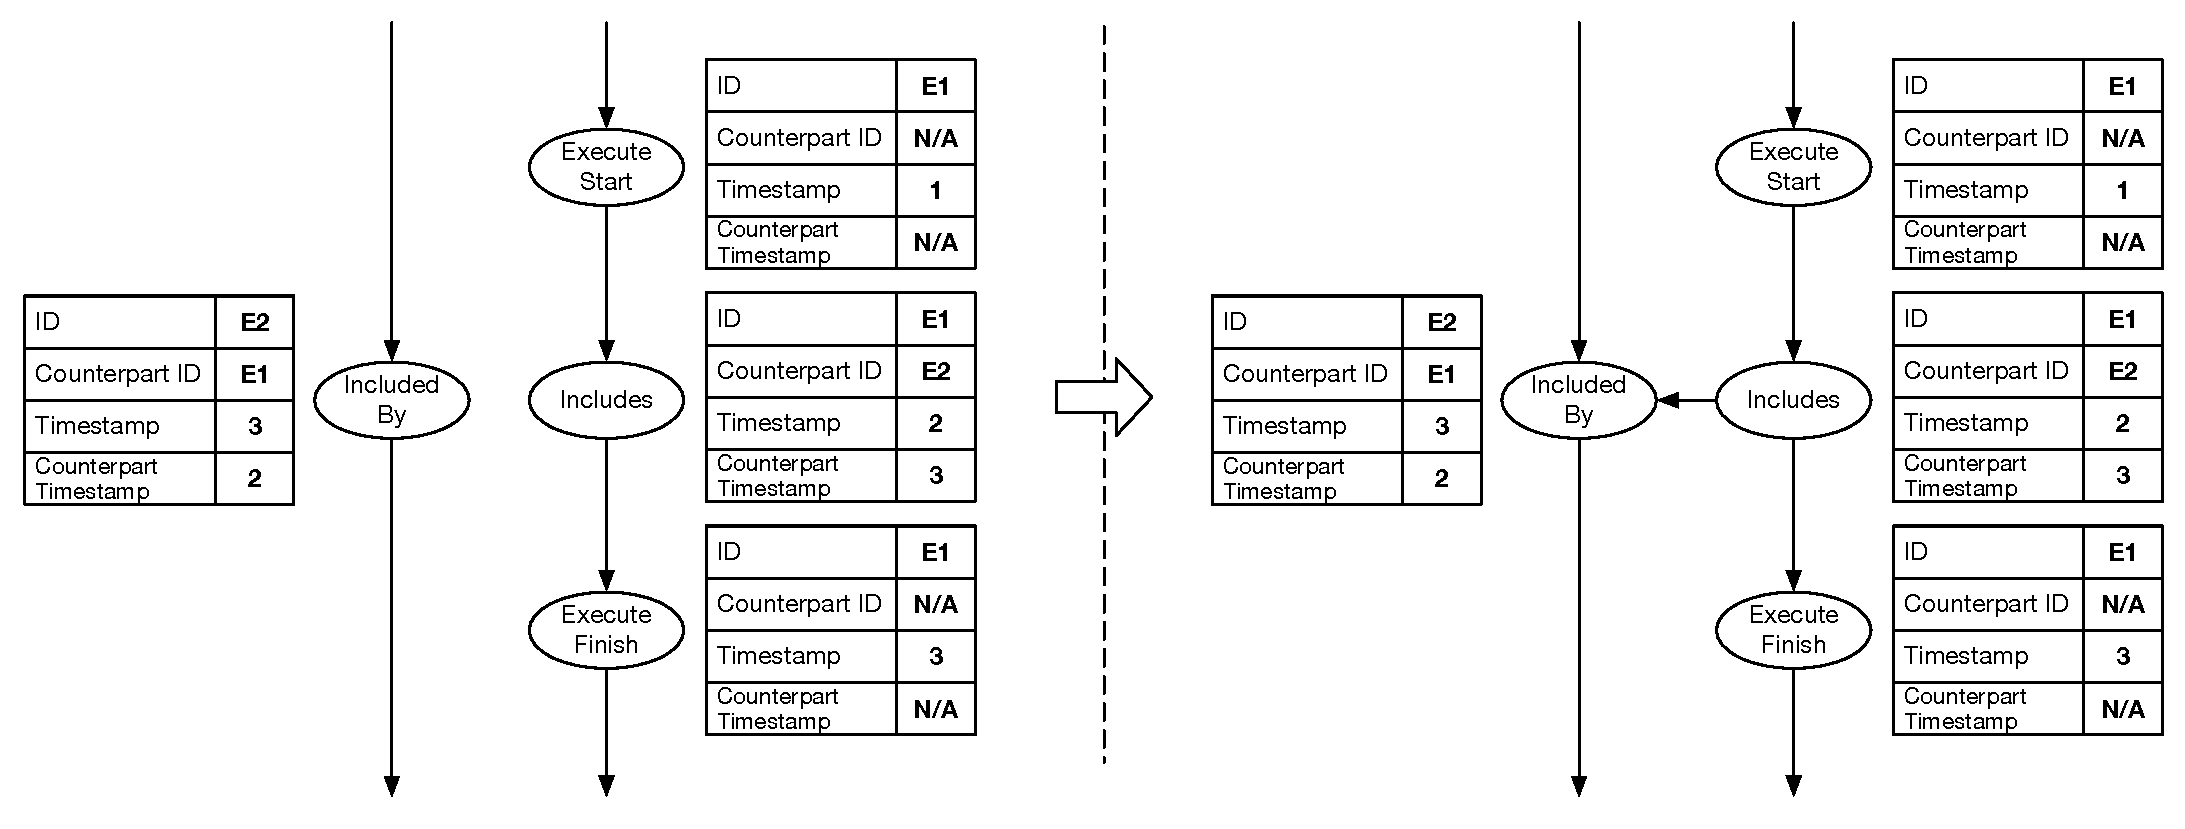
\includegraphics[width=\textwidth]{4connect/images/match-before-after.pdf}
		\caption{Actions of two merged histories before and after being matched.}
		\label{fig:connecting:match-before-after}
	\end{figure}
	
	\todo[inline]{SØREN: Give an example. Pick a tiny DCR
		graph, a distribution of it, and a run for
		it, that you can use as an example
		throughout the report.}
	\todo[inline]{SØREN: That would allow you to here show
		how the history and local history you
		propose would be constructed in that
		instance.}
	\todo[inline]{SØREN: I think you should move the definition
		of valid history up here, and gives
		some form of proof that following the
		algorithm yields a valid history, and
		that you have thus solved the
		consensus problem in the special case
		where no node is malicious/there are
		no byzantine failures.}
    
    \section{Gathering of History}
   
    To merge the histories together it is necessary to acquire access to all the events of the DCR graph first. In a central server system where the server has access to all the individual events it is a trivial task to gather the histories. Simply request the server to get access to all the events and then request the history of each event individually. This method is easy and only relies on the central server to the extent that it in fact returns all the events of the DCR graph. 
    
    Unfortunately central server systems have downfalls. Some of these downfalls include: if the server crashes then it is not possible to acquire access to any of the events, the server has to do the entire workload instead of distributing it out across the peers. Therefore it could be desirable to create a peer to peer based gathering algorithm but this introduced a new set of challenges.
    
    \begin{figure}[H]
		\centering
		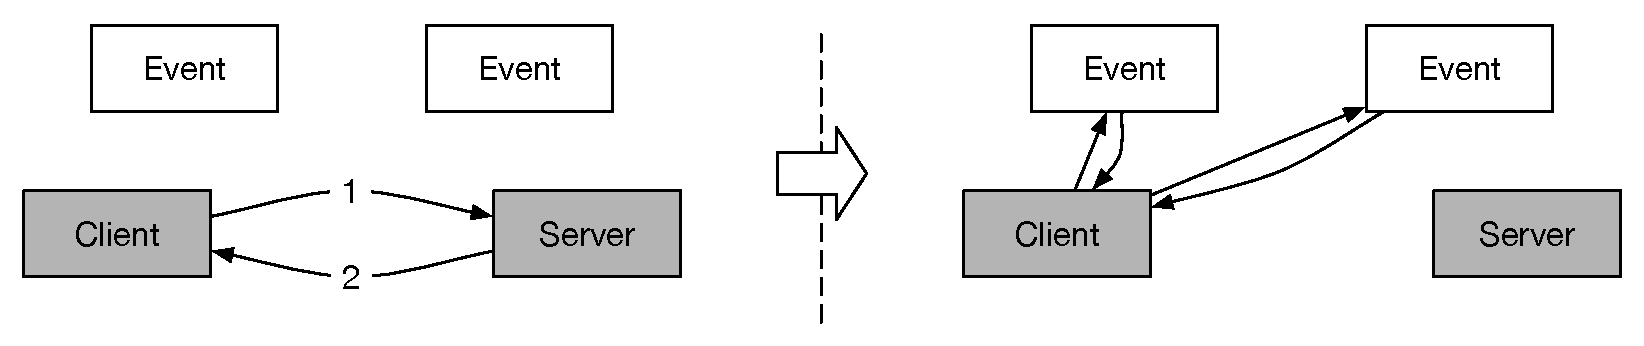
\includegraphics[height=\textheight/6]{4connect/images/server-contacts-events.pdf}
		\caption{The client requesting history from events and receiving it.}
		\label{fig:connecting:server-contacts-events}
	\end{figure}
    
    \subsection{Gathering Without a Central Server}
	Presumed that it is desired to know nothing about the distribution of distributed events in the DCR graph, and therefore have no central all-knowing service handling gathering of history, an alternative approach of gathering history using recursive traversal of the DCR graph can be developed. The following section describes this approach, and the shortcomings it has.   
	
	In order to gather history from a given workflow using recursive traversal, a single starting event must be known. This event will - hopefully - have relations to some other events, and these events will - hopefully - have relations to other events in the DCR graph.
	If the event has no relations, the final gathered history will only contain the history of the contacted event. 
	
	The more connected the DCR graph is, the more complete the gathered history will be. It can therefore not be guaranteed that history from every event will be gathered, if the DCR graph is not fully connected.  
	
	It is desired that any given event in a distributed DCR graph is able to initiate a gathering and production of an order of execution, in cooperation with reachable events in the graph. 
	
	\subsubsection{Analysis}
	If each event only knows a subset of the other events of a workflow, then simply merging the histories of that subset of neighbours will not create a complete history of what has happened up until that moment in time. 
	
	Because of these problems an algorithm which is able to gather information from the entire workflow without knowing all the nodes is developed. Such an algorithm needs to be measured in its ability to reach all reachable events in the graph, as well as its ability to handle relation cycles. 
	
	\subsubsection{The Produce Algorithm}
	Given a DCR graph where all events are not reachable from the starting event, the algorithm should fetch and merge the histories of each event in the graph into one history.
	
	This is accomplished by recursively contacting neighbouring events and asking them for their history while stitching the neighbours' history with its own history. To handle cycles, the use of a trace of previously contacted events is send from each event to the next.
	
	\newpar The implementation uses two lists, called \texttt{request trace} and \texttt{wait for}.
	The algorithm propagates throughout the graph using recursion with checks during execution in order to avoid infinite cycles of requests. 
	
	When an event receives a request for its history, it adds every reachable event from itself to \texttt{wait for}. Then the event crosschecks the event IDs of the \texttt{request trace} and the event's own \texttt{wait for} list. Any event ID in \texttt{wait for} that exists in \texttt{request trace} is removed and the history of the event is returned to the requester. Any remaining events in \texttt{wait for} gets sent requests for history their history with the ID of the event appended to the \texttt{request trace}. 
	
	\subsubsection{Implementation}
	\begin{algorithm}
	\begin{algorithmic}
		\State Event receives request for history with a \texttt{request trace}, $T$.
		\State Event has internal \texttt{wait for}, $W$
		\State
		\State $W\gets W::$ reachable events \Comment Add all reachable events to \texttt{wait for}.
		\If {$W=\emptyset$}
			\Return own history
		\Else
			\State $W\gets W-T$ \Comment Remove every event in $T$ from $W$. Cycles avoided.
			\State $T\gets T::ownID$ \Comment Append own event ID to $T$.
			\State
			\ForAll {$w$ in $W$} 
				\State request history from $w$ with $T$ \Comment Request from neighbours with new \texttt{trace}.
			\EndFor
			\State wait for receiving histories
			\State stitch received histories with own history
			\State
			\Return stitched histories
		\EndIf
	\end{algorithmic}
	\caption{The \textit{\textbf{Fetch}} algorithm}
	\label{alg:fetch}
	\end{algorithm}
	
	\newpar This algorithm is in fact a modified version of the flooding search algorithm for searching in unstructured peer to peer networks. In produce each node visited returns something and not only the searched for node. Furthermore the flooding algorithm is often implemented with a time limit on the search and therefore does not care about cycles, which is handled more effeciently in the produce algorithm.
	
	\begin{figure}[H]
		\centering
		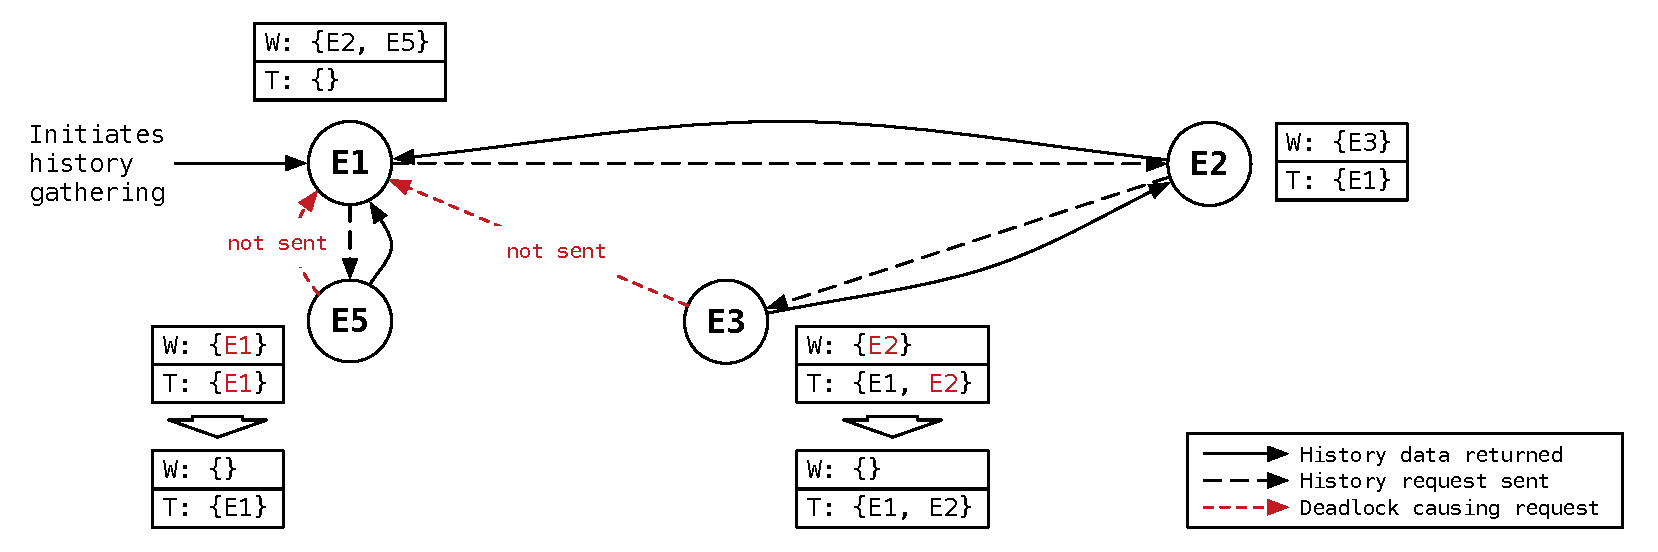
\includegraphics[width=\textwidth]{4connect/images/recursive.pdf}
		\caption{An illustration showing the recursive traversal through a graph. Note the avoidance of creating a deadlock.}
		\label{fig:connecting:recursive}
	\end{figure}
	
	\subsubsection{Correctness}
	Since this algorithm is a modfied version of the flooding algorithm it has most of the same traits with respect to reachability of the algorithm. If there exits a path from the beginning node to all other nodes in the workflow, the algorithm is. 
	
	\subsubsection{Performance}
	This algorithm has a worst case message performance of O(2*N$^2$) where N is the number of events in the system. This occurs when the graph is fully connected, and all events therefore have relations to all other events in the graph. 
	
	Realistically this situation will rarely occur since DCR graphs. \todo{Since wat?}
	
	\newpar Caching history produced of an event before transferring it to a requesting event could improve performance, but presents new problems. 
	
	Certain issues arise if an event with neighbours is the last event in what would have been a produce cycle and due to tracing returns its own local history which would then be cached. This event would then never return the histories of its neighbours if contacted again from a different event, but would instead only return its own history due to caching. 
	
	The neighbours history of the neighbours would then only be produced once, and therefore pass through a single, possibly malicious, node. The lack of redundancy in the system therefore presents an issue when validating histories.
	
	It is therefore necessary to produce redundant histories, which makes caching impossible.
	
	\subsubsection{Issues with Recursive Traversal of the Distributed Graph}
	\todo[inline]{Omformulér afsnit om, at det er tæt på umuligt at validere historik (specielt vha. DCR-regler) uden at kende hele workflowet.}
	
	There is a couple of pitfalls with the algorithm. If malicious events are introduced in the DCR graph, the same problems arise as with the graph where the beginning node had relations with the rest of the graph. 
	
	\newpar That is, if the neighbouring nodes do not know enough of each other, there is no way of making sure that the returned history is correct. Furthermore, this uncertainty is amplified due to the fact that for each contacted event with lacking information, it is possible to tamper with the history of the recursively called events, or even add history of non existent events. Therefore some action must be taken to handle these pitfalls.
	
	The requirements for making it possible to validate the gathered history are described in the following section. 
	
	\begin{figure}[H]
		\centering
		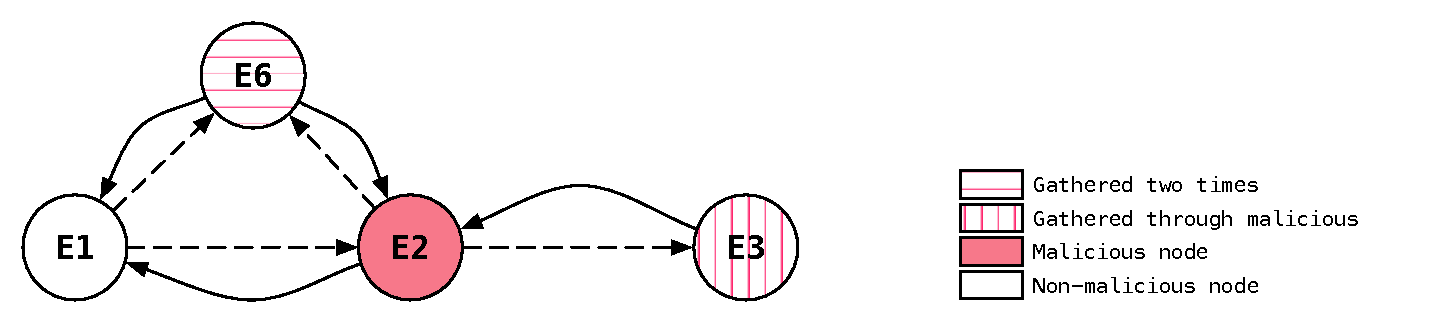
\includegraphics[width=\textwidth]{4connect/images/recursive-evil-node.pdf}
		\caption{A malicious node in a graph. Note that it is not possible to ensure that any history passing through the malicious node is valid.}
		\label{fig:connecting:recursive-evil-node}
	\end{figure}